\section{Übersicht} 

\subsection{Ausgangslage}
Diese Projekt ist für uns Studenten das erste Projekt mit einem externen Auftraggeberin. Jana Kalbermatter ist eine Designerin, die auch die Fachhochschule Nordwestschweiz besucht hat. Ihre Bachleor-Arbeit möchte sie nun realiseren.

Sie hat eine Art Audio-Guide für Museen designt, welcher sie Dojo nennt. Ihre Arbeit beinhaltete das Design des Gehäse und das dazugehörige Konzept. In ihrem Konzept hat sie die Funktionen des Dojo schon relativ genau definiert, jedoch ist sie offen für neue Ideen. Damit stellt sie die Rahmenbedingungen an das Projekt.

Das Konzept sieht einen Köperschallaktor vor, um die Audio-Files abzuspielen. Eine weitere Eigenheit ist auch der Like Button, mit dem man Ausstellungsstücke " Liken" kann. Diese Likes werden am ende des Museumsbesuch zusammengefasst und in einer nicht genauer definierten Form abgegeben. Ansonsten kann der Dojo das was man von einem Audio-Guide erwarten würde.

Unsere Aufgabe besteht darin in einem ersten Schritt einen funktionierenden Prototypen zu bauen. Dieser soll noch nicht so klein werden, dass er in den Dojo hinein passen kann. Die Integration soll in einem zweiten Schritt erfolgen. Dies dürfen jedoch nur die Teams machen, die einen genügend guten Prototypen haben.

\begin{figure}[H]
\begin{center}
	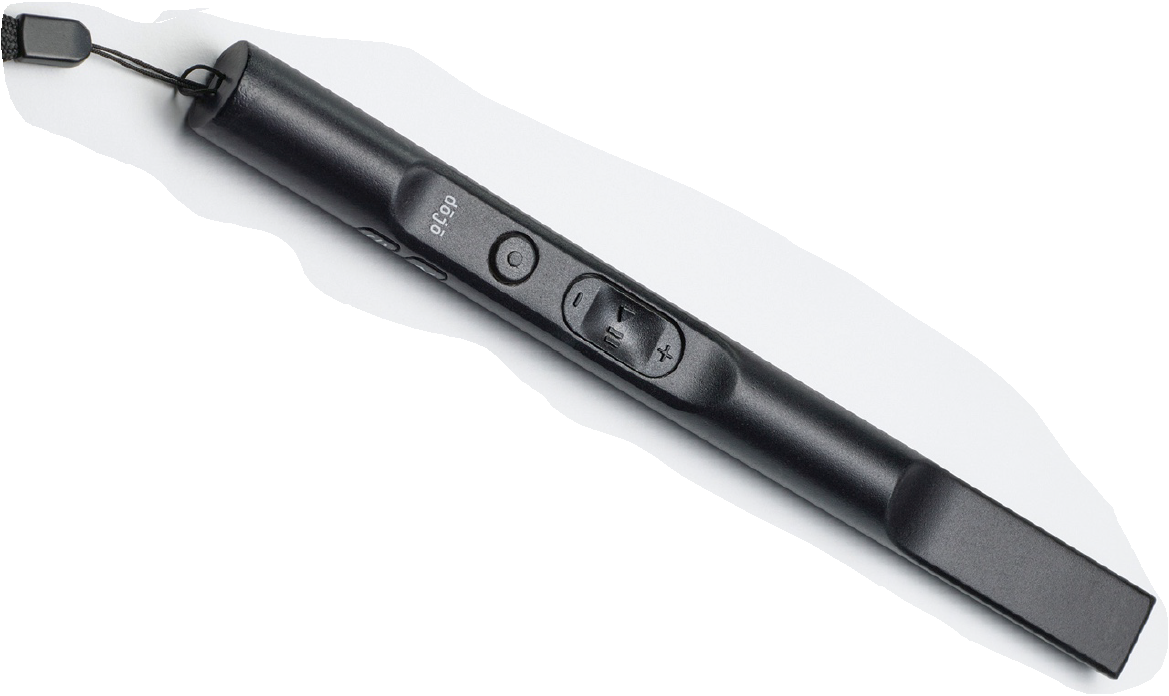
\includegraphics[width=160mm]{data/Ausgangslage_Dojo.png}
	\caption{Konzeptzeichnung des Dojo} %picture caption
	\label{fig:first_layer}
\end{center}
\end{figure}

\pagebreak

\subsection{Projektziele}

\begin{table}[H]
\centering
\begin{tabular}{|c|c|c|}
\hline
\textbf{Nr.:} & \textbf{Muss-Ziele:}                                                  & \textbf{Minimale Anforderungen}                                                                                                                      \\ \hline
1.            & \textbf{Allgemeine}                                                   &                                                                                                                                                      \\ \hline
1.1           & Bedienung                                                             & Die Bedienung des Dojo entspricht dem Lasenheft                                                                                                      \\ \hline
1.2           & Gehäuse                                                               & Das Gehäse wird möglichst wenig verändert                                                                                                            \\ \hline
2.            & \textbf{Audio-Signal}                                                 &                                                                                                                                                      \\ \hline
2.1           & Leistung                                                              & \begin{tabular}[c]{@{}c@{}}Maximale Leistung am\\  Knochenschallaktor 1W/RMS\end{tabular}                                                            \\ \hline
2.2           & Audiodatei                                                            & Audiodatei entsprechend Beacon-ID abspielen.                                                                                                         \\ \hline
2.3           & Aufbereitung                                                          & Filterung (maximale Bandbreite 300Hz-19kHz)                                                                                                          \\ \hline
3.            & \textbf{SD-Karte}                                                     & \begin{tabular}[c]{@{}c@{}}Datentransfer (Daten können gelesen und \\ geschrieben werden)\end{tabular}                                               \\ \hline
4.            & \textbf{Induktives Laden}                                             & die Ladung erfolgt Induktiv                                                                                                                          \\ \hline
5.            & \textbf{Energiespeicher}                                              &                                                                                                                                                      \\ \hline
5.1           & Kapazität                                                             & 500mAh                                                                                                                                               \\ \hline
5.2           & Elektrischer Schutz                                                   & \begin{tabular}[c]{@{}c@{}}Tiefenentladung \& Überladung durch \\ Regelung vermeiden\end{tabular}                                                    \\ \hline
5.3           & Grösse                                                                & 17 x 17 x 55mm                                                                                                                                       \\ \hline
5.4           & Aufladen                                                              & Überladen durch Regelung vermeiden                                                                                                                   \\ \hline
5.5           & Montage                                                               & Montage auf Printlatine                                                                                                                              \\ \hline
6.            & \textbf{Bluetooth}                                                    &                                                                                                                                                      \\ \hline
6.1           & \begin{tabular}[c]{@{}c@{}}Lokalisation \\ Kunstobjekt\end{tabular}   & Erkennung von Beacons auf 3 m Entfernung                                                                                                             \\ \hline
6.2           & \begin{tabular}[c]{@{}c@{}}Identifikation \\ Kunstobjekt\end{tabular} & \begin{tabular}[c]{@{}c@{}}Automatische Auswahl von Beacon mit \\ stärkstem  Signal und Unterscheidung der \\ Beacons mittels Beacon-ID\end{tabular} \\ \hline
              & \textbf{Wunschziele:}                                                 &                                                                                                                                                      \\ \hline
1.            & Daten-Austausch                                                       & \begin{tabular}[c]{@{}c@{}}Bluetooth-Funktionserweiterung um Daten in Dojos\\   Speicher zu laden/löschen\end{tabular}                               \\ \hline
2.            & Lokalisation Dojo                                                     & Sendender Dojo-ID auf Anfrage (vie Bluetooth)                                                                                                        \\ \hline
\end{tabular}
\caption{Projektziele}
\label{Projektziele}
\end{table}

\subsection{Lieferobjekte}
\begin{table}[H]
\centering
\begin{tabular}{|l|l|l|l|}
	\hline 
	Objekt & Form & Empfänger & Termin \\ 
	\hline 
	\begin{tabular}[c]{@{}l@{}}Kriterien der Zusammen- \\arbeit (KIS)\end{tabular} & Als PDF per E-Mail & Arbeitgeber /Fachbetreuer & 20.02.18  \\ 
	\hline 
	Pflichtenheft org. Teil & Als PDF per E-Mail & Arbeitgeber /Fachbetreuer & 13.03.18 \\ 
	\hline 
	Pflichtenheft tech. Teil v1 & Als PDF per E-Mail & Arbeitgeber /Fachbetreuer & 13.03.18 \\ 
	\hline 
	Pflichtenfheft tech. Teil  & Als PDF per E-Mail & Arbeitgeber /Fachbetreuer & 27.03.18 \\ 
	\hline 
	Statusbericht 1 & Als PDF per E-Mail & Arbeitgeber /Fachbetreuer & 27.03.18 \\ 
	\hline 
	Zwischenpräsentation & Englisch mündlich & Projektdozenten & 10.04.18 \\ 
	\hline 
	Statusbericht 2 & Als PDF per E-Mail & Arbeitgeber /Fachbetreuer & 28.04.18 \\ 
	\hline 
	Einleitung und Disposition & Als PDF per E-Mail & R.Dubach & 08.05.18 \\ 
	\hline 
	Statusbericht 3 & Als PDF per E-Mail & Arbeitgeber /Fachbetreuer & 15.05.18 \\ 
	\hline 
	Statusbericht 4 & Als PDF per E-Mail & Arbeitgeber /Fachbetreuer & 05.06.18 \\ 
	\hline 
	Schlusspräsentation & Englisch mündlich & Projektdozenten & 12.06.18 \\ 
	\hline
	Fachbericht & gebundenes Heft & Arbeitgeber /Fachbetreuer & 12.06.18\\ 
	\hline
	PMA-Bericht & gebundenes Heft & P.Buchschacher & 12.06.18 \\ 
	\hline 
	Dojo & Print & Arbeitgeber /Fachbetreuer & 12.06.18 \\ 
	\hline
	Projektdaten & USB-Stick & Arbeitgeber /Fachbetreuer & 12.06.18 \\ 
	\hline
\end{tabular} 
\caption{Lieferobjekte}
\label{Lieferobjekte}
\end{table}
